\section{Wstęp}
Celem projektu była synteza układu regulacji dla systemu wahadła odwróconego na wózku. Wyszczególniono następujące zadania sterowania: doprowadzenie wahadła do górnego, niestabilnego punku równowagi za pomocą algorytmu \textit{swing-up} oraz stabilizację wahadła w niestabilnym punkcie równowagi.

Stanowisko laboratoryjne składa się z wahadła znajdującego się na wózku napędzanym przez silnik DC, enkoderów inkrementalnych sczytujących położenie kątowe wahadła oraz wału silnika. Silnik DC sterowany jest sygnałem PWM. Układ połączony jest z komputerem klasy PC na którym zainstalowany jest system operacyjny Windows, MATLAB R2015b z toolboxami umożliwiającymi automatyczną generację kodu z bloków Simulinka, a także oprogramowanie umożliwiające uruchomienie wygenerowanego kodu w czasie rzeczywistym.


%\begin{figure}
%\centering
%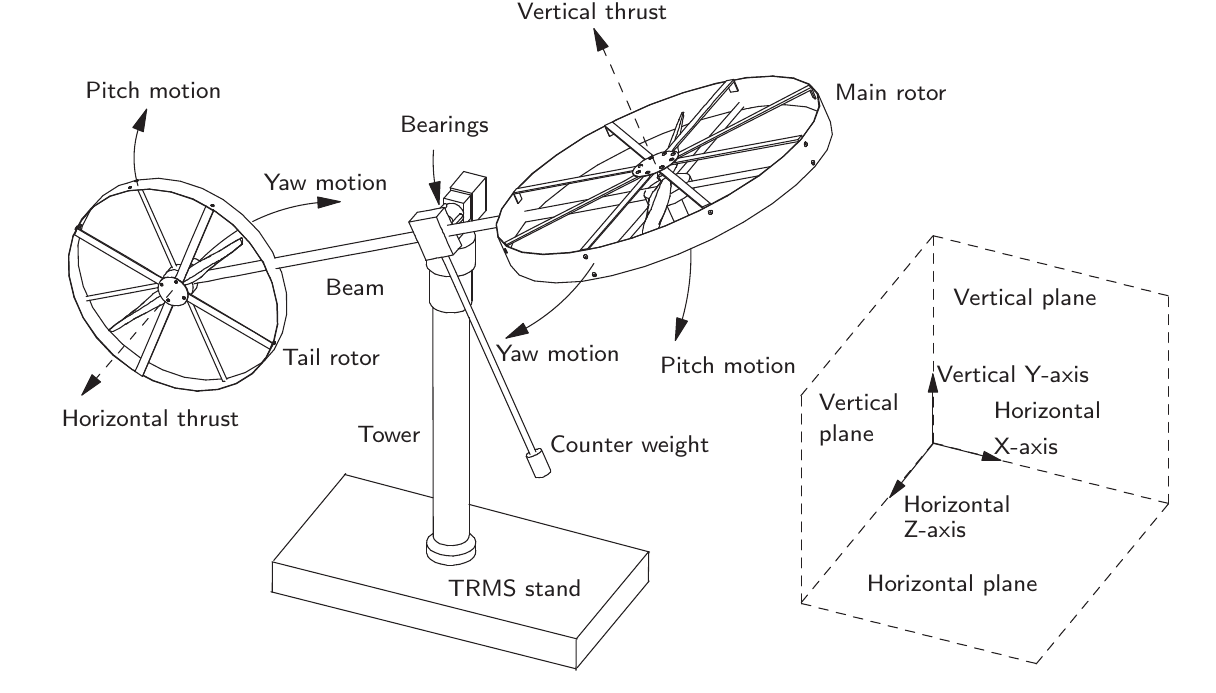
\includegraphics[width=15cm]{obrazy/heli.png}
%\caption{Schemat układu - helikopter na uwięzi}
%\label{fig:heli}
%\end{figure}
